\chapter{Исследовательская часть}
Для формирования системы запросов о пушистости кошек, было необходимо провести опрос среди респондентов и построить функцию принадлежности термам числовых значений признака, описываемого лингвистической переменной~---~пушистостью кошки.
 
В данном разделе приведена анкета, предоставленная респондентам. Также представлены результаты анкетирования и статистической обработки мнений респондентов.

\section{Анкета для респондентов}

Анкета, отправленная респондентам, представляет собой таблицу.

\begin{table}[H]
	\caption{Анкета, отправленная респондентам}
	\begin{tabular}{|c|c|ccccccc|}
		\cline{1-9}
		&                            & \multicolumn{7}{c|}{Количество пушинок на см$^2$ $\xi$, шт.}                                                                                                    \\ \cline{3-9}
		\multirow{-2}{*}{\begin{tabular}[c]{@{}c@{}}№\\ респондента\end{tabular}} & \multirow{-2}{*}{Терм $i$} & \multicolumn{1}{c|}{0} & \multicolumn{1}{c|}{500} & \multicolumn{1}{c|}{1000} & \multicolumn{1}{c|}{5000} & \multicolumn{1}{c|}{10000} & \multicolumn{1}{c|}{15000} & \multicolumn{1}{c|}{20000} \\ \cline{1-9}
		{\color[HTML]{333333} }                                                 & лысая                  & \multicolumn{1}{c|}{}  & \multicolumn{1}{c|}{}     & \multicolumn{1}{c|}{}      & \multicolumn{1}{c|}{}       & \multicolumn{1}{c|}{}       &         \multicolumn{1}{c|}{} & \multicolumn{1}{c|}{}    \\ \cline{2-9}
		{\color[HTML]{333333} }                                                 & плешивая            & \multicolumn{1}{c|}{}  & \multicolumn{1}{c|}{}     & \multicolumn{1}{c|}{}      & \multicolumn{1}{c|}{}       & \multicolumn{1}{c|}{}       &    \multicolumn{1}{c|}{}  & \multicolumn{1}{c|}{}  \\ \cline{2-9}
		{\color[HTML]{333333} }                                                 & волосатая            & \multicolumn{1}{c|}{}  & \multicolumn{1}{c|}{}     & \multicolumn{1}{c|}{}      & \multicolumn{1}{c|}{}       & \multicolumn{1}{c|}{}       &   \multicolumn{1}{c|}{}   & \multicolumn{1}{c|}{} \\ \cline{2-9}
		{\color[HTML]{333333} }                                                 & пушистая                     & \multicolumn{1}{c|}{}  & \multicolumn{1}{c|}{}     & \multicolumn{1}{c|}{}      & \multicolumn{1}{c|}{}       & \multicolumn{1}{c|}{}       &   \multicolumn{1}{c|}{}   & \multicolumn{1}{c|}{} \\ \cline{2-9}
		{\color[HTML]{333333} }                                                 & очень пушистая               & \multicolumn{1}{c|}{}  & \multicolumn{1}{c|}{}     & \multicolumn{1}{c|}{}      & \multicolumn{1}{c|}{}       & \multicolumn{1}{c|}{}       &   \multicolumn{1}{c|}{}  & \multicolumn{1}{c|}{} \\ \cline{2-9}
		\multirow{-6}{*}{{\color[HTML]{333333} 1}}                              & невероятно пушистая         & \multicolumn{1}{c|}{}  & \multicolumn{1}{c|}{}     & \multicolumn{1}{c|}{}      & \multicolumn{1}{c|}{}       & \multicolumn{1}{c|}{}       &   \multicolumn{1}{c|}{}   & \multicolumn{1}{c|}{} \\ \cline{1-9}
	\end{tabular}
\end{table}

\section{Результаты анкетирования}

В таблице \ref{tbl:t1} приведено соответствие между респондентами и их номером.

\begin{table}[H]
	\begin{center}
	\caption{Соответствие № респондента и респондента}
	\label{tbl:t1}
	\begin{tabular}{|c|c|}
		\hline
		№  & Респондент      \\ \hline
		1              & Княжев~А.~В.    \\ \hline
		2              & Глотов~И.~А.   \\ \hline
		3              & Ляпина~Н.~В.    \\ \hline
		4              & Аскарян~К.~А.   \\ \hline
		5              & Обревская~В.~В. \\ \hline
	\end{tabular}
	\end{center}
\end{table}


В таблице \ref{tbl:t2} приведены результаты анкетирования респондентов.

\begin{table}[H]
	\caption{Результаты анкетирования респондентов}
	\label{tbl:t2}
	\begin{tabular}{|c|c|ccccccc|}
		\cline{1-9}
		&                                           & \multicolumn{7}{c|}{Количество пушинок на см$^2$ $\xi$, шт.}                                                                                                                                              \\ \cline{3-9}
		\multirow{-2}{*}{\begin{tabular}[c]{@{}c@{}}№\\ респондента\end{tabular}} & \multirow{-2}{*}{Терм $i$}                & \multicolumn{1}{c|}{0}          & \multicolumn{1}{c|}{500}              & \multicolumn{1}{c|}{1000}                     & \multicolumn{1}{c|}{5000} & \multicolumn{1}{c|}{10000} & \multicolumn{1}{c|}{15000} & \multicolumn{1}{c|}{20000} \\ \cline{1-9}
		{\color[HTML]{333333} }                                                    & лысая                                 & \multicolumn{1}{c|}{1}                        & \multicolumn{1}{c|}{0}                        & \multicolumn{1}{c|}{0}     & \multicolumn{1}{c|}{0}      & \multicolumn{1}{c|}{0}      & \multicolumn{1}{c|}{0}        & \multicolumn{1}{c|}{0} \\ \cline{2-9}
		{\color[HTML]{333333} }                                                    & плешивая                           & \multicolumn{1}{c|}{{\color[HTML]{333333} 0}} & \multicolumn{1}{c|}{{\color[HTML]{333333} 1}} & \multicolumn{1}{c|}{0}     & \multicolumn{1}{c|}{0}      & \multicolumn{1}{c|}{0}      & \multicolumn{1}{c|}{0}        & \multicolumn{1}{c|}{0}  \\ \cline{2-9}
		{\color[HTML]{333333} }                                                    & волосатая                           & \multicolumn{1}{c|}{{\color[HTML]{333333} 0}} & \multicolumn{1}{c|}{{\color[HTML]{333333} 0}} & \multicolumn{1}{c|}{0}     & \multicolumn{1}{c|}{0}      & \multicolumn{1}{c|}{0}      & \multicolumn{1}{c|}{0}       & \multicolumn{1}{c|}{0}  \\ \cline{2-9}
		{\color[HTML]{333333} }                                                    & пушистая                                    & \multicolumn{1}{c|}{{\color[HTML]{333333} 0}} & \multicolumn{1}{c|}{{\color[HTML]{333333} 0}} & \multicolumn{1}{c|}{1}     & \multicolumn{1}{c|}{1}      & \multicolumn{1}{c|}{0}      & \multicolumn{1}{c|}{0}        & \multicolumn{1}{c|}{0}  \\ \cline{2-9}
		{\color[HTML]{333333} }                                                    & очень пушистая                              & \multicolumn{1}{c|}{{\color[HTML]{333333} 0}} & \multicolumn{1}{c|}{{\color[HTML]{333333} 0}} & \multicolumn{1}{c|}{0}     & \multicolumn{1}{c|}{0}      & \multicolumn{1}{c|}{1}      & \multicolumn{1}{c|}{1}        & \multicolumn{1}{c|}{0}  \\ \cline{2-9}
		\multirow{-6}{*}{{\color[HTML]{333333} 1}}                                 & невероятно пушистая                        & \multicolumn{1}{c|}{{\color[HTML]{333333} 0}} & \multicolumn{1}{c|}{{\color[HTML]{333333} 0}} & \multicolumn{1}{c|}{0}     & \multicolumn{1}{c|}{0}      & \multicolumn{1}{c|}{0}      & \multicolumn{1}{c|}{0}        & \multicolumn{1}{c|}{1}  \\ \cline{1-9}
		{\color[HTML]{333333} }                                                    & лысая                                 & \multicolumn{1}{c|}{1}                        & \multicolumn{1}{c|}{1}                        & \multicolumn{1}{c|}{0}     & \multicolumn{1}{c|}{0}      & \multicolumn{1}{c|}{0}      & \multicolumn{1}{c|}{0}        & \multicolumn{1}{c|}{0}  \\ \cline{2-9}
		{\color[HTML]{333333} }                                                    & плешивая                           & \multicolumn{1}{c|}{{\color[HTML]{333333} 0}} & \multicolumn{1}{c|}{{\color[HTML]{333333} 0}} & \multicolumn{1}{c|}{1}     & \multicolumn{1}{c|}{0}      & \multicolumn{1}{c|}{0}      & \multicolumn{1}{c|}{0}        &      \multicolumn{1}{c|}{0}                 \\ \cline{2-9}
		{\color[HTML]{333333} }                                                    & волосатая                           & \multicolumn{1}{c|}{{\color[HTML]{333333} 0}} & \multicolumn{1}{c|}{{\color[HTML]{333333} 0}} & \multicolumn{1}{c|}{0}     & \multicolumn{1}{c|}{1}      & \multicolumn{1}{c|}{0}      & \multicolumn{1}{c|}{0}        &            \multicolumn{1}{c|}{0}           \\ \cline{2-9}
		{\color[HTML]{333333} }                                                    & пушистая                                    & \multicolumn{1}{c|}{{\color[HTML]{333333} 0}} & \multicolumn{1}{c|}{{\color[HTML]{333333} 0}} & \multicolumn{1}{c|}{0}     & \multicolumn{1}{c|}{0}      & \multicolumn{1}{c|}{1}      & \multicolumn{1}{c|}{0}        & \multicolumn{1}{c|}{0}                       \\ \cline{2-9}
		{\color[HTML]{333333} }                                                    & очень пушистая                              & \multicolumn{1}{c|}{{\color[HTML]{333333} 0}} & \multicolumn{1}{c|}{{\color[HTML]{333333} 0}} & \multicolumn{1}{c|}{0}     & \multicolumn{1}{c|}{0}      & \multicolumn{1}{c|}{0}      & \multicolumn{1}{c|}{1}        & \multicolumn{1}{c|}{0}                       \\ \cline{2-9}
		\multirow{-6}{*}{{\color[HTML]{333333} 2}}                                 & невероятно пушистая                        & \multicolumn{1}{c|}{{\color[HTML]{333333} 0}} & \multicolumn{1}{c|}{{\color[HTML]{333333} 0}} & \multicolumn{1}{c|}{0}     & \multicolumn{1}{c|}{0}      & \multicolumn{1}{c|}{0}      & \multicolumn{1}{c|}{0}        & \multicolumn{1}{c|}{1}                       \\ \cline{1-9}
		{\color[HTML]{333333} }                                                    & лысая                                 & \multicolumn{1}{c|}{1}                        & \multicolumn{1}{c|}{0}                        & \multicolumn{1}{c|}{0}     & \multicolumn{1}{c|}{0}      & \multicolumn{1}{c|}{0}      & \multicolumn{1}{c|}{0}        & \multicolumn{1}{c|}{0}  \\ \cline{2-9}
		{\color[HTML]{333333} }                                                    & {\color[HTML]{333333} плешивая}    & \multicolumn{1}{c|}{{\color[HTML]{333333} 0}} & \multicolumn{1}{c|}{{\color[HTML]{333333} 1}} & \multicolumn{1}{c|}{1}     & \multicolumn{1}{c|}{0}      & \multicolumn{1}{c|}{0}      & \multicolumn{1}{c|}{0}        & \multicolumn{1}{c|}{0}                       \\ \cline{2-9}
		{\color[HTML]{333333} }                                                    & {\color[HTML]{333333} волосатая}    & \multicolumn{1}{c|}{{\color[HTML]{333333} 0}} & \multicolumn{1}{c|}{{\color[HTML]{333333} 0}} & \multicolumn{1}{c|}{0}     & \multicolumn{1}{c|}{1}      & \multicolumn{1}{c|}{0}      & \multicolumn{1}{c|}{0}        & \multicolumn{1}{c|}{0}                       \\ \cline{2-9}
		{\color[HTML]{333333} }                                                    & {\color[HTML]{333333} пушистая}             & \multicolumn{1}{c|}{{\color[HTML]{333333} 0}} & \multicolumn{1}{c|}{{\color[HTML]{333333} 0}} & \multicolumn{1}{c|}{0}     & \multicolumn{1}{c|}{0}      & \multicolumn{1}{c|}{1}      & \multicolumn{1}{c|}{0}        & \multicolumn{1}{c|}{0}                       \\ \cline{2-9}
		{\color[HTML]{333333} }                                                    & {\color[HTML]{333333} очень пушистая}       & \multicolumn{1}{c|}{{\color[HTML]{333333} 0}} & \multicolumn{1}{c|}{{\color[HTML]{333333} 0}} & \multicolumn{1}{c|}{0}     & \multicolumn{1}{c|}{0}      & \multicolumn{1}{c|}{0}      & \multicolumn{1}{c|}{1}        & \multicolumn{1}{c|}{0}                       \\ \cline{2-9}
		\multirow{-6}{*}{{\color[HTML]{333333} 3}}                                 & {\color[HTML]{333333} невероятно пушистая} & \multicolumn{1}{c|}{{\color[HTML]{333333} 0}} & \multicolumn{1}{c|}{{\color[HTML]{333333} 0}} & \multicolumn{1}{c|}{0}     & \multicolumn{1}{c|}{0}      & \multicolumn{1}{c|}{0}      & \multicolumn{1}{c|}{0}        & \multicolumn{1}{c|}{1}                       \\ \cline{1-9}
		{\color[HTML]{333333} }                                                    & лысая                                 & \multicolumn{1}{c|}{1}                        & \multicolumn{1}{c|}{1}                        & \multicolumn{1}{c|}{0}     & \multicolumn{1}{c|}{0}      & \multicolumn{1}{c|}{0}      & \multicolumn{1}{c|}{0}        & \multicolumn{1}{c|}{0}  \\ \cline{2-9}
		{\color[HTML]{333333} }                                                    & {\color[HTML]{333333} плешивая}    & \multicolumn{1}{c|}{{\color[HTML]{333333} 0}} & \multicolumn{1}{c|}{{\color[HTML]{333333} 0}} & \multicolumn{1}{c|}{0}     & \multicolumn{1}{c|}{0}      & \multicolumn{1}{c|}{0}      & \multicolumn{1}{c|}{0}        & \multicolumn{1}{c|}{0}                       \\ \cline{2-9}
		{\color[HTML]{333333} }                                                    & {\color[HTML]{333333} волосатая}    & \multicolumn{1}{c|}{{\color[HTML]{333333} 0}} & \multicolumn{1}{c|}{{\color[HTML]{333333} 0}} & \multicolumn{1}{c|}{1}     & \multicolumn{1}{c|}{1}      & \multicolumn{1}{c|}{1}      & \multicolumn{1}{c|}{0}        & \multicolumn{1}{c|}{0}                       \\ \cline{2-9}
		{\color[HTML]{333333} }                                                    & {\color[HTML]{333333} пушистая}             & \multicolumn{1}{c|}{{\color[HTML]{333333} 0}} & \multicolumn{1}{c|}{{\color[HTML]{333333} 0}} & \multicolumn{1}{c|}{0}     & \multicolumn{1}{c|}{0}      & \multicolumn{1}{c|}{0}      & \multicolumn{1}{c|}{1}        & \multicolumn{1}{c|}{0}                       \\ \cline{2-9}
		{\color[HTML]{333333} }                                                    & {\color[HTML]{333333} очень пушистая}       & \multicolumn{1}{c|}{{\color[HTML]{333333} 0}} & \multicolumn{1}{c|}{{\color[HTML]{333333} 0}} & \multicolumn{1}{c|}{0}     & \multicolumn{1}{c|}{0}      & \multicolumn{1}{c|}{0}      & \multicolumn{1}{c|}{0}        & \multicolumn{1}{c|}{1}                       \\ \cline{2-9}
		\multirow{-6}{*}{{\color[HTML]{333333} 4}}                                 & {\color[HTML]{333333} невероятно пушистая} & \multicolumn{1}{c|}{{\color[HTML]{333333} 0}} & \multicolumn{1}{c|}{{\color[HTML]{333333} 0}} & \multicolumn{1}{c|}{0}     & \multicolumn{1}{c|}{0}      & \multicolumn{1}{c|}{0}      & \multicolumn{1}{c|}{0}        & \multicolumn{1}{c|}{0}                       \\ \cline{1-9}
		{\color[HTML]{333333} }                                                    & лысая                                 & \multicolumn{1}{c|}{1}                        & \multicolumn{1}{c|}{0}                        & \multicolumn{1}{c|}{0}     & \multicolumn{1}{c|}{0}      & \multicolumn{1}{c|}{0}      & \multicolumn{1}{c|}{0}        & \multicolumn{1}{c|}{0}  \\ \cline{2-9}
		{\color[HTML]{333333} }                                                    & {\color[HTML]{333333} плешивая}    & \multicolumn{1}{c|}{{\color[HTML]{333333} 0}} & \multicolumn{1}{c|}{{\color[HTML]{333333} 1}} & \multicolumn{1}{c|}{0}      & \multicolumn{1}{c|}{0}      & \multicolumn{1}{c|}{0}      & \multicolumn{1}{c|}{0}        & \multicolumn{1}{c|}{0}                       \\ \cline{2-9}
		{\color[HTML]{333333} }                                                    & {\color[HTML]{333333} волосатая}    & \multicolumn{1}{c|}{{\color[HTML]{333333} 0}} & \multicolumn{1}{c|}{{\color[HTML]{333333} 0}} & \multicolumn{1}{c|}{1}     & \multicolumn{1}{c|}{0}      & \multicolumn{1}{c|}{0}      & \multicolumn{1}{c|}{0}        & \multicolumn{1}{c|}{0}                       \\ \cline{2-9}
		{\color[HTML]{333333} }                                                    & {\color[HTML]{333333} пушистая}             & \multicolumn{1}{c|}{{\color[HTML]{333333} 0}} & \multicolumn{1}{c|}{{\color[HTML]{333333} 0}} & \multicolumn{1}{c|}{0}     & \multicolumn{1}{c|}{1}      & \multicolumn{1}{c|}{0}      & \multicolumn{1}{c|}{0}        & \multicolumn{1}{c|}{0}                       \\ \cline{2-9}
		{\color[HTML]{333333} }                                                    & {\color[HTML]{333333} очень пушистая}       & \multicolumn{1}{c|}{{\color[HTML]{333333} 0}} & \multicolumn{1}{c|}{{\color[HTML]{333333} 0}} & \multicolumn{1}{c|}{0}     & \multicolumn{1}{c|}{0}      & \multicolumn{1}{c|}{0}      & \multicolumn{1}{c|}{0}        & \multicolumn{1}{c|}{0}                       \\ \cline{2-9}
		\multirow{-6}{*}{{\color[HTML]{333333} 5}}                                 & {\color[HTML]{333333} невероятно пушистая} & \multicolumn{1}{c|}{{\color[HTML]{333333} 0}} & \multicolumn{1}{c|}{{\color[HTML]{333333} 0}} & \multicolumn{1}{c|}{0}     & \multicolumn{1}{c|}{0}      & \multicolumn{1}{c|}{1}      & \multicolumn{1}{c|}{1}        & \multicolumn{1}{c|}{1}                       \\ \cline{1-9}
	\end{tabular}
\end{table}



\section{Функция принадлежности термам числовых значений признака,  описываемого лингвистической переменной}

Из результатов анкетирования респондентов получим функцию принадлежности термам числовых значений признака,  описываемого лингвистической переменной.

\begin{table}[H]
	\begin{center}
	\caption{Таблица значений функции принадлежности}
	\begin{tabular}{|c|c|c|c|c|c|c|c|c|c|}
		\cline{1-9}
		\multirow{2}{*}{лысая}          &  $\mu_j(\xi)$ & 5   & 2   & 0   & 0   & 0   & 0   &  0\\ \cline{2-9}
		& $F_j(\xi)$ & 1.0 & 0.4 & 0.0 & 0.0 & 0.0 & 0.0 &  0.0\\ \cline{1-9}
		\multirow{2}{*}{плешивая}    &  $\mu_j(\xi)$ & 0   & 3   & 2   & 0   & 0   & 0   &  0\\ \cline{2-9}
		& $F_j(\xi)$ & 0.0 & 0.6 & 0.4 & 0.0 & 0.0 & 0.0 & 0.0 \\ \cline{1-9}
		\multirow{2}{*}{волосатая}    &  $\mu_j(\xi)$ & 0   & 0   & 2   & 3   & 1   & 0   &  0\\ \cline{2-9}
		& $F_j(\xi)$ & 0.0 & 0.0 & 0.4 & 0.6 & 0.2 & 0.0 & 0.0 \\ \cline{1-9}
		\multirow{2}{*}{пушистая}             &  $\mu_j(\xi)$ & 0   & 0   & 1   & 2   & 2   & 1   & 1 \\ \cline{2-9}
		& $F_j(\xi)$ & 0.0 & 0.0 & 0.2 & 0.4 & 0.4 & 0.2 & 0.2 \\ \cline{1-9}
		\multirow{2}{*}{очень пушистая}       &  $\mu_j(\xi)$ & 0   & 0   & 0   & 0   & 1   & 3   & 1 \\ \cline{2-9}
		& $F_j(\xi)$ & 0.0 & 0.0 & 0.0 & 0.0 & 0.2 & 0.6 & 0.2 \\ \cline{1-9}
		\multirow{2}{*}{невероятно пушистая} &  $\mu_j(\xi)$ & 0   & 0   & 0   & 0   & 1   & 1   &  3\\ \cline{2-9}
		& $F_j(\xi)$ & 0.0 & 0.0 & 0.0 & 0.0 & 0.2 & 0.2 & 0.6 \\ \cline{1-9}
	\end{tabular}
	\end{center}
\end{table}

В таблице выше $\mu_j(\xi) = \sum\limits_{k=1}^K a^{k}_{ji}$, $F_j(\xi)= \frac{S_j(\xi)}{K}$, где $K$ -- количество респондентов.

На рисунках \ref{img:plot1} и \ref{img:plot2} представлены графики, отражающий функциональную зависимость $F_j(\xi)$.

\begin{table}[H]
	\centering
	\begin{tabular}{p{1\linewidth}}
		\centering
		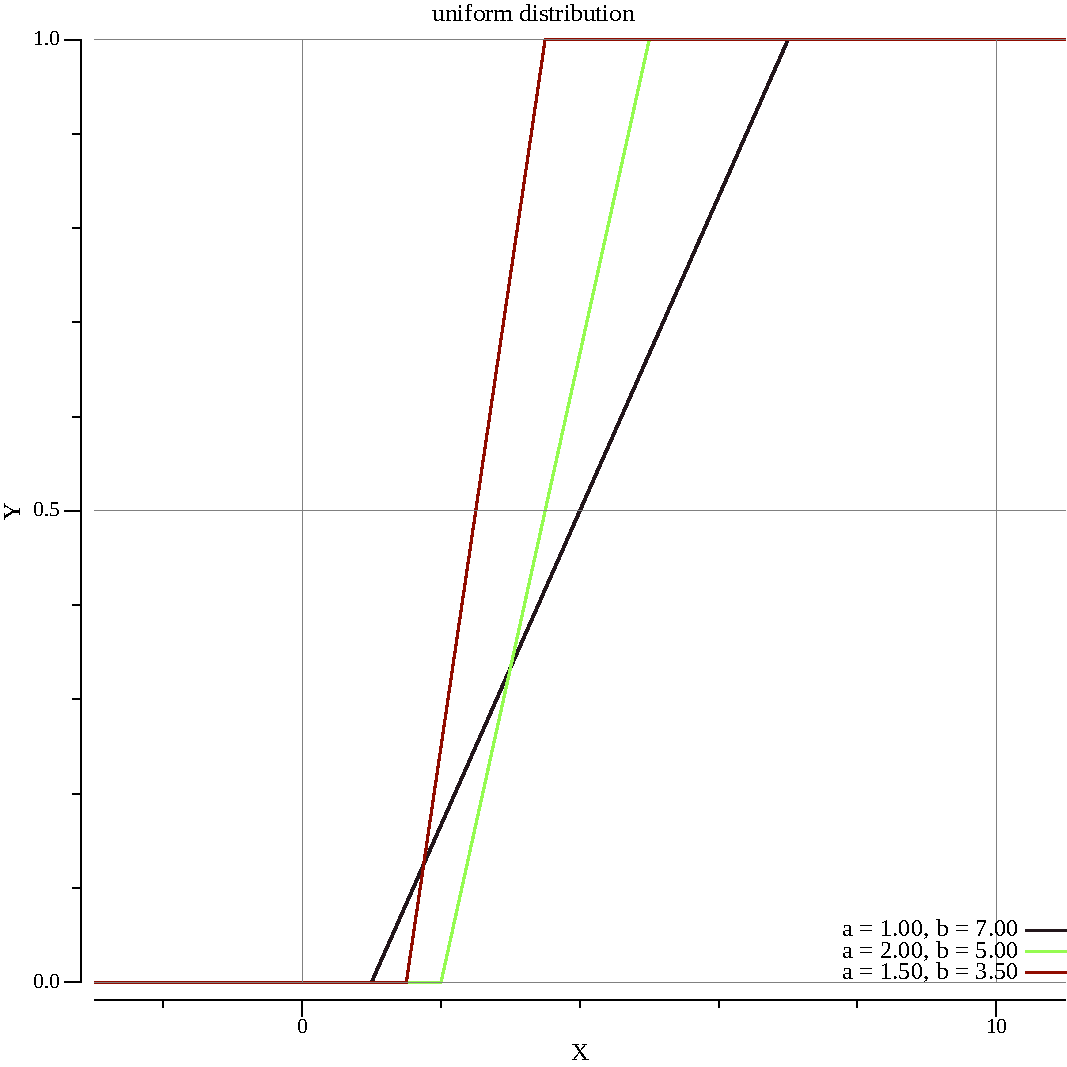
\includegraphics[width=0.9\linewidth]{all.pdf}
		\captionof{figure}{Функциональная зависимость $F_j(\xi)$ (от 0 до 5000 по оси абсцисс)}
		\label{img:plot1}
	\end{tabular}
\end{table}

\begin{table}[H]
	\centering
	\begin{tabular}{p{1\linewidth}}
		\centering
		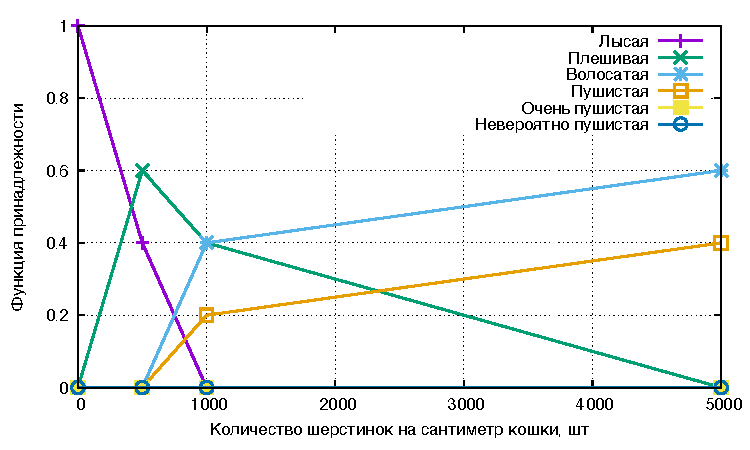
\includegraphics[width=0.9\linewidth]{start.pdf}
		\captionof{figure}{Функциональная зависимость $F_j(\xi)$}
		\label{img:plot2}
	\end{tabular}
\end{table}

\section{Соответствие признаков и диапазонов значений}

В таблице \ref{tbl:t3} приведено соответствие между признаками и диапазонами значений пушистости кошки.

\begin{table}[H]
	\begin{center}
	\caption{Соответствие между термами и диапазонами значений пушистости кошки}
	\label{tbl:t3}
	\begin{tabular}{|c|c|}
		\hline
		Признак            & Диапазон \\ \hline
		лысая          &  $\left[0;417\right]$        \\ \hline
		плешивая    &       $\left[418;1000\right]$    \\ \hline
		волосатая    &     $\left[1001;7500\right]$      \\ \hline
		пушистая             &    $\left[7501;11667\right]$     \\ \hline
		очень пушистая       &        $\left[11668;17500\right]$   \\ \hline
		невероятно пушистая &    $\left[17500;20000\right]$       \\ \hline
	\end{tabular}
	\end{center}
\end{table}
